\documentclass[11pt]{article}

\usepackage[letterpaper,margin=0.75in]{geometry}
\usepackage{booktabs}
\usepackage{graphicx}
\usepackage{listings}

\setlength{\parindent}{1.4em}

\begin{document}

\lstset{
  language=Python,
  basicstyle=\small,          % print whole listing small
  keywordstyle=\bfseries,
  identifierstyle=,           % nothing happens
  commentstyle=,              % white comments
  stringstyle=\ttfamily,      % typewriter type for strings
  showstringspaces=false,     % no special string spaces
  numbers=left,
  numberstyle=\tiny,
  numbersep=5pt,
  frame=tb,
}

\title{Lab 5 Report - Distance Vector Routing}

\author{Jonathan George}

\date{April 14th, 2015}

\maketitle

This report explains an implementation for distance vector routing protocol for Bene. This allows it to dynamically route packets across an arbitrary network of simulated nodes. We used the Bene simulator to run experiments to show the correctness of this protocol




\section{Routing Protocol}

The routing protocol implemented in this lab was fairly simple. Each node starts our only knowing about it's own links. Every 30 seconds it broadcasts a message containing it's distance vector table. These packets have a TTL of 1, so they only reach the closest neighbors. Upon receiving a distance vector table from a neighbor, the node updates it's own distance vector table with the information given. At this time, it also sets up it's own forwarding table. 

The routing protocol is designed to allow for links to be taken down and have the rest of the nodes adjust their paths to handle the change. After 3 rounds of broadcasts without hearing from a node, then the node is assumed lost and it's information is deleted from the table. One important thing to note is this can lead to a count to infinity problem. This will be demonstrated later on

The distance vector message sent between the nodes had the following format:

['n1', (1, 0), (2, 1), (3, 1), (4, 2), (5, 2), (6, 3), (7, 3), (8, 4)]

n1 represents the starting node. The tuples which follow contain the link address and the cost to get to that link from the starting node. This message format allows for the receiving node to know who sent the message and also the costs from that node to the various nodes it has already discovered.

Distance vector tables were initialized with the following code segments.

\begin{lstlisting}
def init_vector_table(self):
    for link in self.links:
        self.vector_table[link.address] = 0
\end{lstlisting}

The messages once received were processed by the node with the following code. As can be seen, we parse the message and then if the link has been seen before we compare each cost with the current cost. Otherwise we just add the new link to the distance vector table.

\begin{lstlisting}
def update_vector_table(self, vector_table_msg):
    hostname = vector_table_msg[0]
    for tup in vector_table_msg[1:]:
        dest = tup[0]
        value = tup[1] + 1 #add one to account for travel time to this node.
        
        if dest in self.vector_table.keys():
            if value < self.vector_table[dest] :
                self.vector_table[dest] = value
                self.add_forwarding_entry(dest,self.get_link(hostname))
            if value <= self.vector_table[dest]:
                self.TTL_links[dest] = 3
        else:
            self.vector_table[dest] = value
            self.add_forwarding_entry(dest,self.get_link(hostname))
            self.TTL_links[dest] = 3
\end{lstlisting}

An importance aspect which can be seen above is the TTL Links dictionary which keeps track of how long it has been since the last time a node was seen. The following code is called once each phase before sending out the vector table.

\begin{lstlisting}
def decrement_TTL(self):
    for link in self.TTL_links.keys():
        self.TTL_links[link] -= 1
        if self.TTL_links[link] <= 0:
            #pop is a safer way to delete entries in a dictionary.
            self.TTL_links.pop(link,None)
            self.vector_table.pop(link,None)
            self.forwarding_table.pop(link,None) 
\end{lstlisting}


\section{Experiments}

In the following section we will describe each of the experiments we ran to ensure that our implementation is correct.

\subsection{Five Nodes in a Row}

In this first section we ran a test which showed that a chain of five nodes could discover each other and a message could be sent from the first node to the last. The network configuration looked like the following.



\begin{lstlisting}
#
#  n1 --- n2 --- n3 --- n4 --- n5
# 
\end{lstlisting}

Our expereiment printed out the trace of the packet from n1 to n5 and also the final vector tables for each node. The output was the following.

\centerline{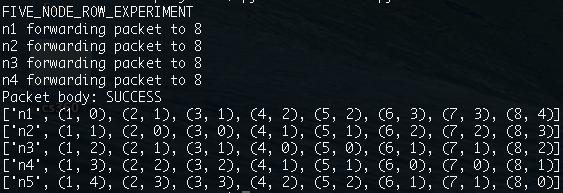
\includegraphics[width=16cm]{five_node_row.png}}

As can be seen by the trace, the experiment was a success and each node learned of every other node. The message was also sent successfully.

\subsection{Five Nodes in a Loop}
In this section we tested to ensure that the shortest path was taken from one node to another. We also tested how the system reacts when one node is taken down. Again, here is the network configuration

\begin{lstlisting}
#
#  n1 --- n2 --- n3 --- n4 --- n5
#   \__________________________/
# 
\end{lstlisting}

The experiment first sends a packet from n1 to n5. Then the link between n1 and n5 is taken down. Then another packet is sent to n5 a short time later. The distance vector tables are printed out before and after the link is taken down.

\centerline{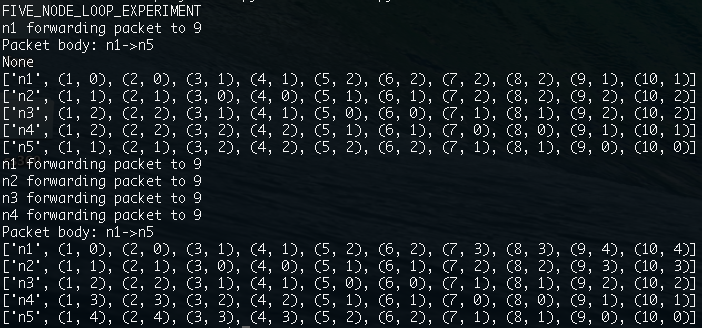
\includegraphics[width=16cm]{five_node_loop.png}}

It can be seen that before the link is taken down that the costs line up with taking the shortest path. The first packet likewise travels directly to n5. After the link is taken down, the link all adjust correctly and the packet is sent through n2,n3 and n4 to reach n5. 

\subsection{Fifteen Node Mesh}

In this experiment, we will test a larger mesh to ensure that taking down links will still function correctly. The configuration for this mesh is the following.

\begin{lstlisting}
#
#       --- n7 --- n8
#      /    |       |
#    n9     |       |
#      \--- n6     n2 -- n14 -- n15
#            \    /  \   /
#             \  /    \ /
#      n10 --- n1     n3
#               |      |
#               |      |
#              n4 --- n5 -- n13
#               |      |
#               |      |
#              n11    n12
#
\end{lstlisting}

This experiment first sends a node from n1 to n5. As expected it takes the shorter route through n4. Then we take down n4 and see that it will travel through n2 and n3 instead. We finally bring the link back up once more and this allows us once again to travel through n4. The following is the output from the experiment.

\centerline{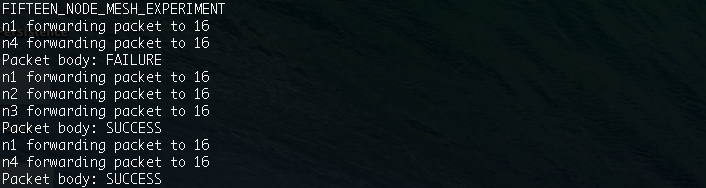
\includegraphics[width=16cm]{fifteen_node_mesh.png}}

This experiment also functions as expected.

\subsection{The Count to Infinity Problem}

In this experiment, we explored the possablity and existence of the count to infinity problem. This problem occurs when a link expires, but other links trust false positive messages from neighbors which claim they can reach it. This causes the neighbors to go back and forth about who can actually reach the node and they start to count upwards with one another. In this experiment, we will use the five nodes in a row configuration. After the links have established themselves, we will take down n1's connecting links. This will cause n2 and n3 to contest how to reach n1 as they begin to time out. We printed out the vector table at increasing increments to see how the cost to reach one grows larger and larger regardless of the fact that they cannot reach it.

\centerline{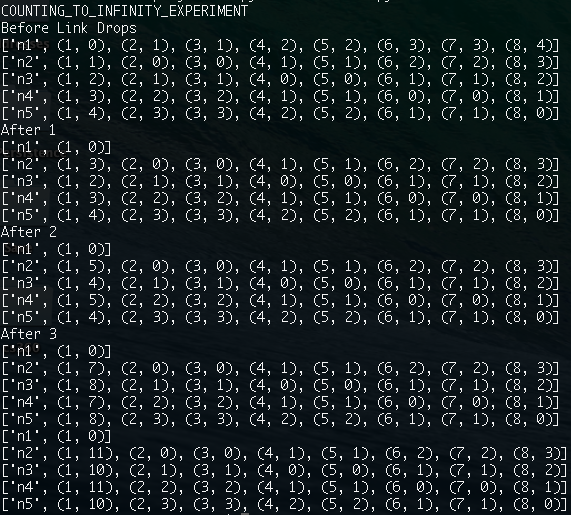
\includegraphics[width=16cm]{count_infinity.png}}

This output shows that n2 starts out with a cost distance to n1 of 1. However, once the link goes down and it times out. Then it immediately hears about n1 from n3 and sets it's value to 3. This pattern continues and the nodes began to count upwards forever. This could be solved in a few different ways, but we did not undertake this.


\subsection{TCP behavior}

After running all of these experiment, it was important to ensure that TCP from previous labs still worked correctly. This was just a simple test of sending a packet between n1 and n13 in the fifteen node mesh configuration. The following graphs show that TCP behavior was still correct.

\centerline{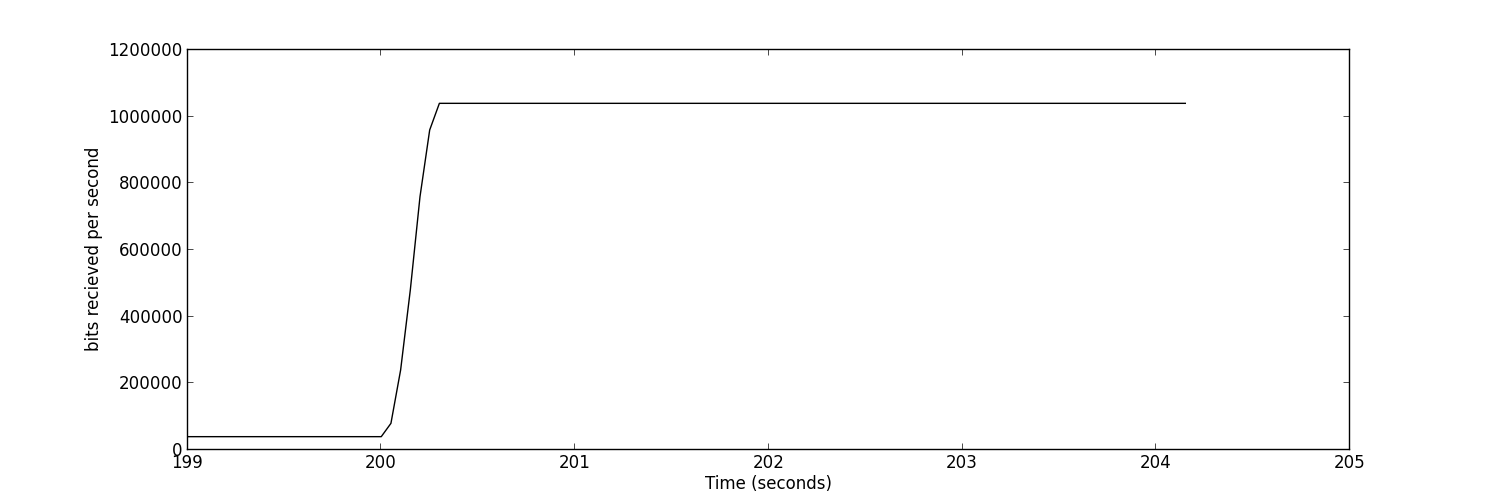
\includegraphics[width=16cm]{plot_rate_one.png}}

\centerline{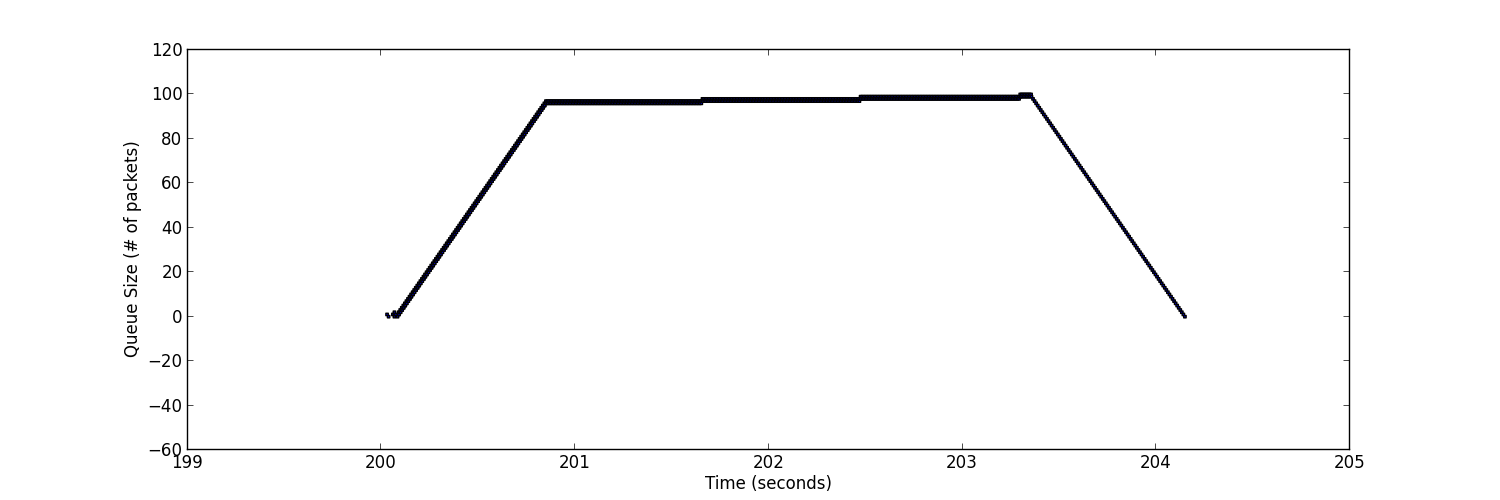
\includegraphics[width=16cm]{queue_time_one.png}}

\centerline{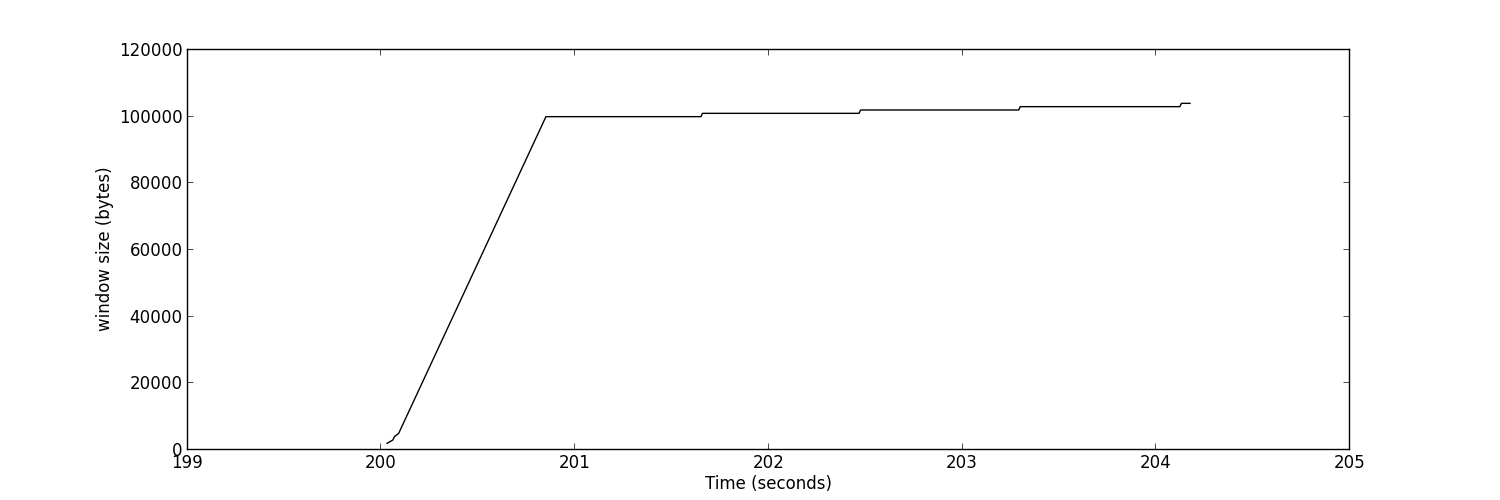
\includegraphics[width=16cm]{window_time_one.png}}

\end{document}




















